\documentclass[11pt]{article}
\usepackage[a4paper, margin=1in]{geometry}
\usepackage{amsfonts,amsmath,amssymb,mathtools}
\usepackage[none]{hyphenat}
\usepackage{fancyhdr}
\usepackage{graphicx}
\usepackage[parfill]{parskip} %Removes indentation on new paragraph 
\usepackage{tkz-euclide}

\pagestyle{fancy}
\fancyhead{} %clears default header
\fancyfoot{} %clears default footer
\fancyhead[L]{Ethan Lim} %\slshape makes itallics

\begin{document}

\section*{Question 5}
The in-center of a triangle is the point equidistant from the triangles
sides.
% , and we take for granted the fact that the in-center can be equivalently defined
% as the point where the three angle bisectors of the triangle intersect.

\begin{center}
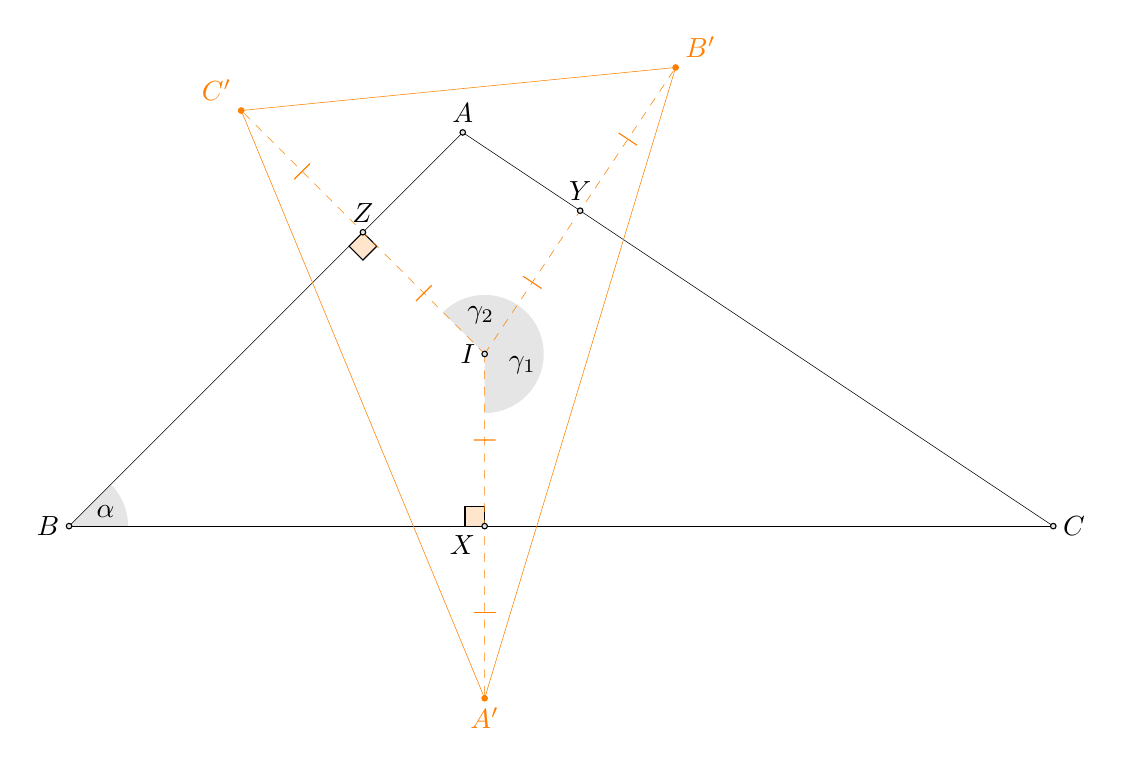
\begin{tikzpicture}[scale=2.5]
	% initial points
	\tkzDefPoint(2,2){A}
	\tkzDefPoint(0,0){B}
	\tkzDefPoint(5,0){C}

	% incenter
	\tkzDefTriangleCenter[in](A,B,C)
	\tkzGetPoint{I}

	% reflected points
	\tkzDefPointBy[reflection=over B--C](I)
	\tkzGetPoint{A'}
	\tkzDefPointBy[reflection=over A--C](I)
	\tkzGetPoint{B'}
	\tkzDefPointBy[reflection=over A--B](I)
	\tkzGetPoint{C'}

	% mark right angles
	\tkzInterLL(B,C)(I,A')
	\tkzGetPoint{X}
	\tkzInterLL(A,C)(I,B')
	\tkzGetPoint{Y}
	\tkzInterLL(A,B)(I,C')
	\tkzGetPoint{Z}
	
	\tkzMarkRightAngle[fill=orange!20,size=0.1](B,X,I)
	\tkzMarkRightAngle[fill=orange!20,size=0.1](B,Z,I)

	% angles
	\tkzFillAngle[size=0.3,fill=gray!20](C,B,A)
	\tkzFillAngle[size=0.3,fill=gray!20](A',I,B')
	\tkzFillAngle[size=0.3,fill=gray!20](B',I,C')

	\tkzLabelAngle[pos=0.2](C,B,A){$\alpha$}
	\tkzLabelAngle[pos=0.2](A',I,B'){$\gamma_1$}
	\tkzLabelAngle[pos=0.2](B',I,C'){$\gamma_2$}

	% draw lines
	\tkzDrawSegment(A,B)
	\tkzDrawSegment(B,C)
	\tkzDrawSegment(C,A)

	\tkzDrawSegment[orange,dashed](I,A')
	\tkzDrawSegment[orange,dashed](I,B')
	\tkzDrawSegment[orange,dashed](I,C')

	% draw points
	\tkzDrawPoints(A,B,C,X,Y,Z,I)
	\tkzDrawPoints[orange](A',B',C')
	\tkzDrawSegment[orange](A',B')
	\tkzDrawSegment[orange](B',C')
	\tkzDrawSegment[orange](C',A')

	% label points
	\tkzLabelPoint[above](A){$A$}
	\tkzLabelPoint[left](B){$B$}
	\tkzLabelPoint[right](C){$C$}
	\tkzLabelPoint[below left](X){$X$}
	\tkzLabelPoint[above](Y){$Y$}
	\tkzLabelPoint[above](Z){$Z$}
	\tkzLabelPoint[left](I){$I$}
	\tkzLabelPoint[color=orange,below](A'){$A'$}
	\tkzLabelPoint[color=orange,above right](B'){$B'$}
	\tkzLabelPoint[color=orange,above left](C'){$C'$}

	% mark lines
	\tkzMarkSegment[color=orange,pos=0.5,mark=|](I,X)
	\tkzMarkSegment[color=orange,pos=0.5,mark=|](I,Y)
	\tkzMarkSegment[color=orange,pos=0.5,mark=|](I,Z)
	\tkzMarkSegment[color=orange,pos=0.5,mark=|](X,A')
	\tkzMarkSegment[color=orange,pos=0.5,mark=|](Y,B')
	\tkzMarkSegment[color=orange,pos=0.5,mark=|](Z,C')

\end{tikzpicture}
\end{center}

Let $\alpha=\angle ABC$, $\gamma_1=\angle A'IB'$ and $\gamma_2=\angle B'IC'$, let $X=BC\cap A'I$, $Y=AC\cap B'I$, $Z=AB\cap C'I$. 

Since $C'$ is the reflection of the point $I$ about the line $AB$, it follows that $\angle IZB=90^\circ$ and $|IZ|=|ZC'|$, similarly, $\angle IXC=90^\circ$, $|IX|=|XA'|$, $\angle IYA=90^\circ$ and $|IY|=|YB'|$. Since $IX$ is perpendicular to $BC$, it follows that the distance from $I$ to the line $BC$ is equal to the length of the segment $IX$, by similar reasoning, the distance from $I$ to $AC$ is $|IY|$, and the distance from $I$ to $AB$ is $|IZ|$, since $I$ is the in-center of $\triangle ABC$, it follows that $|IX|=|IY|=|IZ|$. From this it follows that $|IA'|=|IB'|=|IC'|$.

Looking at quadrilateral $BXIZ$, we can deduce that $\angle XIZ=180^\circ-\alpha$, hence $\gamma_1+\gamma_2=360^\circ-\angle XIZ=180^\circ+\alpha$. Now $\triangle IC'B'$ is isosceles, so $\angle IB'C'=\displaystyle\frac{180^\circ-\gamma_2}{2}$, similarly, $\angle IB'A'=\displaystyle\frac{180^\circ-\gamma_1}{2}$. Hence
\begin{align*}
	\angle A'B'C'&=\angle IB'C'+\angle IB'A'\\
	&=\frac{360^\circ-(\gamma_1+\gamma_2)}{2}\\
	&=\frac{360^\circ-(180^\circ+\alpha)}{2}\\
	&=90^\circ-\frac{\alpha}{2}\\
	&=90^\circ-\frac{\angle ABC}{2}\\
\end{align*}
Hence $\angle A'B'C'$ depends on $\angle ABC$ only, and therefore does not depend on $\angle BAC$
\end{document}